\section{General GPU Architecture}
\label{sec:gpu}

The Graphical Processing Unit (GPU) is a device which is attached to a host machine.
This means that the GPU is an attached piece of hardware, which then is a work horse that works together with the CPU to perform computations.
We present \cref{fig:sm example} as a reference for this section.

\begin{figure}[htb]
  \centering
  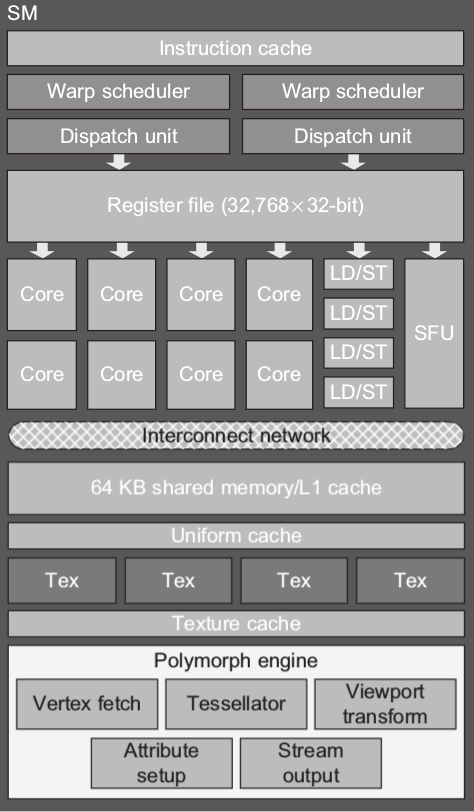
\includegraphics[width=.5\textwidth]{graphics/images/cropped-cuda-sm.png}
  \caption{Example of a Streaming Multiprocessor for reference~\cite{farber2011cuda}}
  \label{fig:sm example}
\end{figure}

A GPU's basic building block is the streaming multiprocessor (SM), which is independently responsible for its own resources, cores, and memory.
By making each SM independent memory access and computation are performed faster, because there is not global memory or special units that are shared among all the hardware.
Each SM has Single Instruction Multiple Data (SIMD) Arithmetic Logic Units (ALU), which are commonly referred to as the cores.
These cores will all run the same instruction, but may use different data.

The work given to the GPU is distributed to the SMs by the Giga-Thread global scheduler, which knows when the SMs are busy.
CUDA-enabled devices are categorised by their compute capability which describes the amount of threads each block can have.
Threads actually perform computations.
They are organised into blocks and grids.
These are described further in \cref{chap:software}.

The SMs receive instructions in a cache and warp schedulers distribute the work to the cores, so the instructions can be executed.
Each thread has access to its own registers, which is called its local memory.
Each SM has shared memory for high-speed data sharing between threads in a block.
The GPU as a whole has memory called global memory, which is accessible by all the GPU's SMs.

Furthermore, an SM has load/store (LD/ST) units and Special Function Units (SFU).
LD/STs calculate source and destination addresses and loads/store data as needed.
SFUs execute special functions, e.g. sin, sqrt, etc.
Each SFU executes one instruction per thread per clock.
SFUs can perform an operation while it is communicating with another thread.
Compared to the SIMD cores, the SFUs are designed specifically to perform their designated functions, and the SIMD cores are general purpose cores.

% good warp answers:  http://stackoverflow.com/questions/11816786/why-bother-to-know-about-cuda-warps
%                     http://stackoverflow.com/questions/10460742/how-do-cuda-blocks-warps-threads-map-onto-cuda-cores
A warp is a block of 32 SIMD threads, and they are the basic unit for scheduling work in the SMs.
To maximize the utilisation of the GPU the developer must make sure that these warp sizes are considered when executing code.
If one does not consider the warp size and randomly schedules tasks, then the programs might have many idle threads that do nothing.
If this is the case, then the GPU is not utilised to its optimal capacity~\cite{fermi2009nvidia}.

\subsection{Hardware Specific Numbers}
\label{sec:hardware specific numbers}

Throughout this report, we will be using the Tesla K40 GPU~\cite{teslak402013nvidia}.
For future reference \cref{tab:tesla k40 specs} presents the specifications for our GPU device.
In \cref{ap:tesla k40 specifications} we walk through how we found the specifications for our device.
\todo{is L1 cache used for shared memory?}

\begin{table}[htb]
  \centering
  \begin{tabular}{l r}
    \toprule
    item                        & limit \\
    \midrule
    warp size                   & \SI{32}{} \\
    max threads / block         & \SI{1024}{} \\
    total cores                 & \SI{2880}{} \\
    registers / block           & \SI{65536}{} \\
    constant memory             & \SI{65536}{B} \\
    L1 cache / block            & \SI{49152}{B}  \\
    L2 cache / core             & \SI{1572864}{B}  \\
    global memory               & \SI{12079136768}{B} \\
    \bottomrule
  \end{tabular}
  \caption{Tesla K40 GPU's specifications}
  \label{tab:tesla k40 specs}
\end{table}

Furthermore, the maximum dimension of grids and blocks are presented in \cref{tab:tesla k40 grid and block}.

\begin{table}[htb]
  \centering
  \begin{tabular}{r r r r}
    \toprule
    item & x & y & z \\
    \midrule
    block size & \SI{1024}{} & \SI{1024}{} & \SI{64}{} \\
    grid size  & \SI{2147483647}{} & \SI{65535}{} & \SI{65535}{} \\
    \bottomrule
  \end{tabular}
  \caption{Tesla K40 GPU's block and grid sizes}
  \label{tab:tesla k40 grid and block}
\end{table}
